\documentclass{article}

\usepackage{kpfonts}
\usepackage{graphicx}
\usepackage{cite}
\usepackage{url}
\usepackage{footnote}
\usepackage[bottom]{footmisc}
\usepackage{epstopdf}
\usepackage[section]{placeins}
\usepackage{xcolor}

\newcommand{\code}[1]{\texttt{#1}}

\author{David~Grelsson \\ \texttt{davidgrelsson@gmail.com}}
\date{\today}
\title{Interactive Ray Tracing Utilizing GPGPU}

\begin{document}

\maketitle


\section{Introduction}
\label{sec:Introduction}
Ray tracing is a technique for rendering images by simulating light rays. A ray is shot from the eye through each pixel
in the scene. Intersection tests are performed to find the object closest to the eye. The intersection point can then
be determined to be in shadow or illuminated by shooting a ray from the intersection point to each light source. If the
ray reaches the light source the intersection point is illuminated, otherwise it is shadowed. If the intersected object
has a reflective material a new ray is shot from the intersection point and the process described above is repeated.
This continues until an object with a diffuse material is hit or a maximum trace depth is reached.

Ray tracing allows for a higher degree of visual realism than other rendering techniques such as 
rasterization~\cite{GPUPro3RayTracer}. However ray tracing also comes with a higher computational cost resulting in poor 
performance when it comes to real time applications. Interactive ray tracing has been possible for some time for simpler
scenes~\cite{RealTimeRendering} but does not perform well enough for real-time applications such as video games~\cite{Friedrich:2006}.

Since each ray can be evaluated independently from all other rays ray tracing greatly benefits from a parallel implementation,
where adding more processors often results in a near linear performance increase~\cite{RealTimeRendering}. With GPUs becoming
more powerful and more importantly, more programmable~\cite{MassivelyParallelProcessors} there now is a way to more easily exploit
the high level of parallelism that ray tracers exhibit.

In this study a ray tracer that utilizes the compute shader in DirectX 11 is implemented. Performance tests are then conducted
to see how resolution, trace depth, number of light sources, thread block sizes and number of triangles affect performance.



\section{Implementation}
\label{sec:Implementation}
The ray tracer in this study was implemented using C++ and the Compute Shader in DirectX 11. It can render triangle and sphere
primitives that each can have their own material attached to them. It follows the ray tracing implementation described by
Arturo Garcia et al.~\cite{GPUPro3RayTracer} where the necessary initialization at startup and updates between frames are
handled by the C++ code executing on the CPU and the ray tracing part of the application is handled by three separate
stages running on the Compute Shader.


\subsection{Primary Ray Stage}
This is the start of the algorithm and its purpose is to generate the rays that are shot into the scene. A ray is created
for each pixel with its origin the same as the camera position and the direction determined by the position of the pixel.

Besides origin and direction each ray also has the id of the last primitive to have been hit by the ray. This is to be able
to prevent the ray from hitting the same primitive again due to numerical errors when it is being bounced. The ray also has
a reflective factor that is modified by the material of the primitive that was hit last and determines how much the current
bounce will contribute to the final color of the pixel. 

The primary ray stage is executed once at the start of each frame and in addition to generating rays the primary ray stage
is also responsible for clearing the result buffer from the results generated in the previous frame.


\subsection{Intersection Stage}
The intersection stage determines which primitive, if any, the ray has hit. It uses the more naive approach of testing each
ray against all primitives in the scene and returning the best intersection i.e. the one closest to the ray origin.

The intersection information i.e. the distance of the intersection point from the ray origin, the id of the primitive that
was intersected and the barycentric coordinates of the intersection point on that primitive are stored in a buffer to
later be used in the next stage of the algorithm.

The intersection stage is executed multiple times each frame, once for each bounce.


\subsection{Color Stage}
This is where the color of each pixel is determined. Using the id of the intersected primitive and the barycentric coordinates
from the previous stage the position, surface normal and texture coordinates of the intersected point can be calculated. The intersected
primitives material information can then be accessed and its texture sampled to get a base color value.

Secondary rays are then created for each light source in the scene. The intersect position is used as the origin for each ray and
the direction is determined by the position of each light source. New intersection tests are performed where, again using the
naive approach, all secondary rays are tested against all the primitives in the scene to determine if the point is lit or in shadow.
Based on the results of the intersection tests lighting calculations are performed to determine the color of the intersected
point. This color value is then modified by the primary ray's reflective factor and added to the result buffer.

The primary ray is then reflected. Its origin being set to the intersected points position. Its direction changed using 
the HLSL intrinsic function \code{reflect} and the intersect point's surface normal. And finally the ray's reflective factor is
modified by the intersected primitive's specular value.

\subsection{Light Sources}
All the light sources used in this application are point lights. The lights are defined in the C++ code on the CPU and
accessed by the GPU using a \textit{Shader Resource View}. Using the \code{DeviceContext::Map} method the lights can be
updated by the CPU between shader calls updating properties such as e.g. position to create moving light sources.


\subsection{Primitives, Materials and Textures}
The application is capable of rendering triangles and spheres. Triangles are loaded from a Wavefront obj file. 
Each triangle consists of three vertices and a material index. Each vertex in turn consists of a position, normal and
texture coordinates. Spheres consists of a center position, radius and a material index. Materials are loaded from
Wavefront mtl files and stored in an array that is accessed by the material indices on the triangles and spheres. 

Each material has a texture associated with it. Textures are loaded into a \code{Texture2DArray} object and can be accessed
by the same indices as the materials. Triangles, spheres, materials and textures are made available to the GPU as
\textit{Shader Resource Views}.
%Sphere primitives defined in the code. Accessible on gpu via Shader resource view.
%
%Triangle primitives loaded from wavefront obj file. Each triangle primitive consists of three vertices and a material id.
%Accessible on gpu via Shader resource view.
%
%Materials loaded from wavefront obj mtl file. Accessible on gpu via Shader resource view.
%
%Textures loaded using DirectX Toolkit. Accessible on gpu via Texture2DArray, same index as material.



\section{Method}
\label{sec:Method}
The scene that was rendered by the ray tracer consisted of two boxes and a sphere.
One of the boxes was large, acting as a room containing the smaller box and the sphere where the rays could bounce around
(see figure~\ref{fig:screenshot_01}).

Several tests were run where the execution time of each shader stage was measured for different configurations of the ray tracer. 
The following properties were altered to see how they would affect performance:

\begin{itemize}
    \centering
    \item Screen Resolution
    \item Thread Block Size
    \item Trace Depth
    \item Number of Lights
    \item Number of Triangles
\end{itemize}

Each test used the configuration displayed in table~\ref{tab:standardConfig} as a base line. For example when different screen resolutions
where tested the thread block size, trace depth, number of lights and number of triangles always had the values presented in table~\ref{tab:standardConfig}.

\begin{table}
    \centering
    \def\arraystretch{1.5}
    \begin{tabular}{c|c}
        Resolution       & 1280x1024 \\
        \hline
        Thread Block Size & 16x16 \\
        \hline
        Trace Depth      & 3 \\
        \hline
        Number of Lights & 4 \\
        \hline
        Number of Triangles & 24 \\
        \hline
    \end{tabular}
    \caption{Standard configuration of the ray tracer. \label{tab:standardConfig}}
\end{table}

A more interesting approach would have been to test all different permutations to see how the different values affect each other.
But considering the scope of this study there was a desire to keep the data generated by the test to a more manageable level.

During the tests the camera was kept in a stationary position in one of the corners overlooking the room (see figure~\ref{fig:screenshot_01}).
Each test ran for five minutes collecting data.

\begin{figure}[h!tbp]
    \centering
    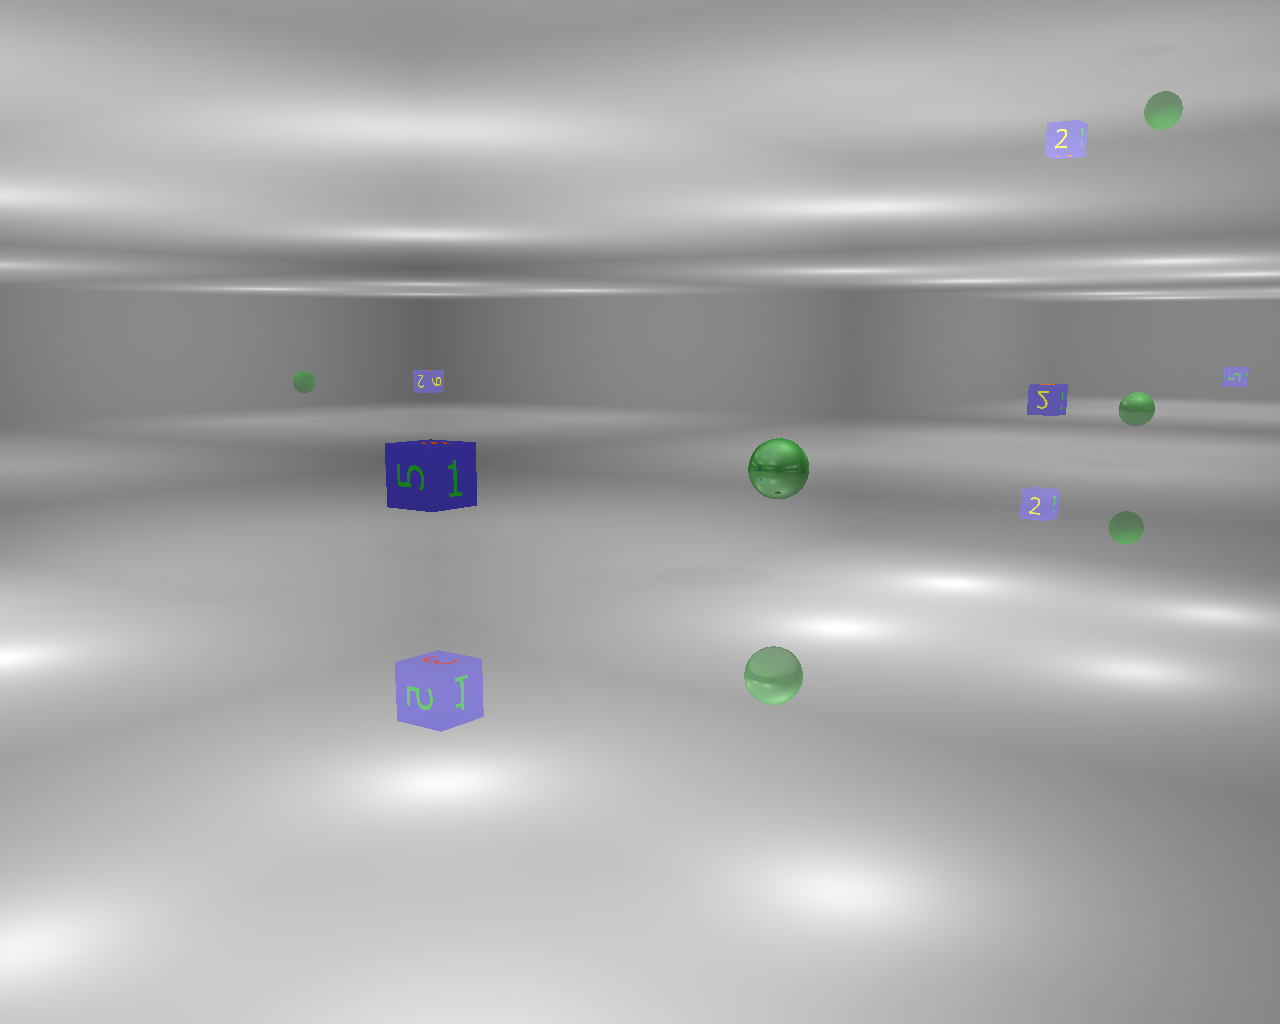
\includegraphics[width=0.9\columnwidth]{Figures/screenshot_01.png}
    \caption{Screenshot of the scene used in the experiment. \label{fig:screenshot_01}}
\end{figure}



\section{Results}
\label{sec:Results}
In this section the results of the tests described in section~\ref{sec:Method} are presented. The values in the tables and
graphs are the average values of the execution time for each shader stage: Primary Ray, Intersection and Color.


\subsection{Resolution}

\begin{figure}[h!tbp]
\centering
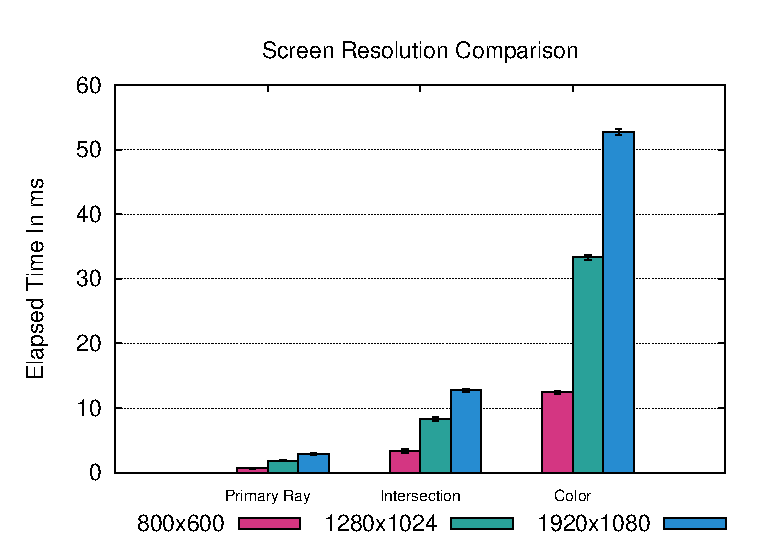
\includegraphics[width=1.0\columnwidth]{Figures/resolution.eps}
\caption{Average elapsed time in ms for different resolutions. \label{fig:resolution}}
\end{figure}

\begin{table}[h!btp]
\centering
\begin{tabular}{c|c|c|c|c}
    Resolution  & Primary Ray & Intersection & Color & Total \\ [2pt]
\hline
    800x600 & 0.689549 & 3.31683 & 12.4687 & 16.475079 \\
\hline
    1280x1024 & 1.84867 & 8.29189 & 33.3089 & 43.44946 \\
\hline
    1920x1080 & 2.87235 & 12.7814 & 52.7882 & 68.44195 \\
\hline
% Mean Value, Standard Deviation
\end{tabular}
\caption{Average elapsed time in ms for different resolutions. \label{tab:ResultsResolution}}
\end{table}


\subsection{Trace Depth}

\begin{figure}[h!tbp]
\centering
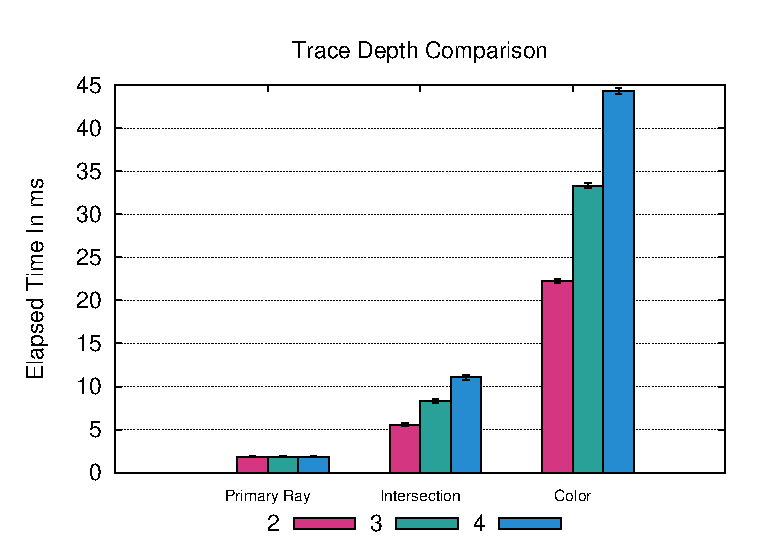
\includegraphics[width=1.0\columnwidth]{Figures/traceDepth.eps}
\caption{Average elapsed time in ms for different trace depths. \label{fig:traceDepth}}
\end{figure}


\begin{table}[h!btp]
\centering
\begin{tabular}{c|c|c|c|c}
    Trace Depth & Primary Ray & Intersection & Color & Total \\ [2pt]
\hline
    2 & 1.85042 & 5.53545 & 22.2733 & 29.65917 \\
\hline
    3 & 1.84899 & 8.30323 & 33.3126 & 43.46482 \\
\hline
    4 & 1.85413 & 11.0674 & 44.3539 & 57.27543 \\
\hline
% Mean Value, Standard Deviation
\end{tabular}
\caption{Average elapsed time in ms for different trace depths. \label{tab:ResultsTraceDepth}}
\end{table}


\subsection{Lights}

\begin{figure}[h!tbp]
    \centering
    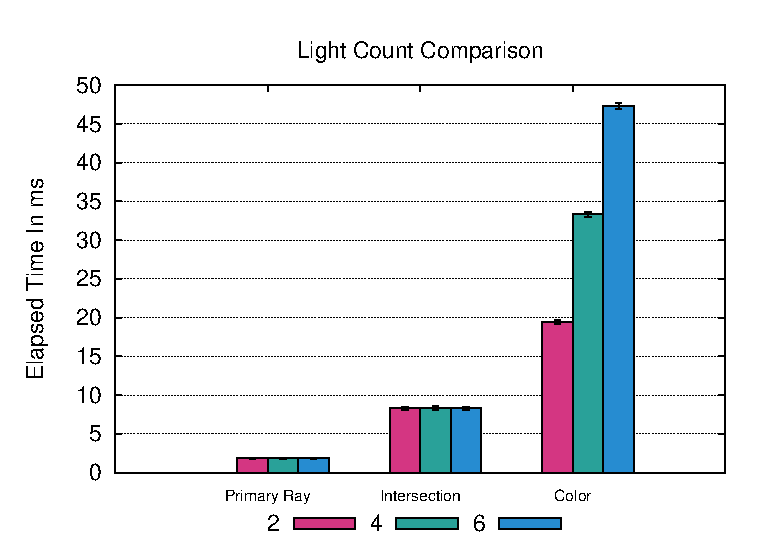
\includegraphics[width=1.0\columnwidth]{Figures/lightcount.eps}
    \caption{Average elapsed time in ms for different number of lights. \label{fig:lightCount}}
\end{figure}

\begin{table}[h!btp]
\centering
\begin{tabular}{c|c|c|c|c}
    Light Count & Primary Ray & Intersection & Color & Total \\ [2pt]
\hline
    2 & 1.84708 & 8.28784 & 19.4441 & 29.57902 \\
\hline
    4 & 1.85202 & 8.30228 & 33.3158 & 43.4701 \\
\hline
    6 & 1.86065 & 8.30864 & 47.3375 & 57.50679 \\
\hline
% Mean Value, Standard Deviation
\end{tabular}
\caption{Average elapsed time in ms for different number of lights. \label{tab:ResultsNumberOfLights}}
\end{table}


\subsection{Thread Blocks}

\begin{figure}[h!tbp]
    \centering
    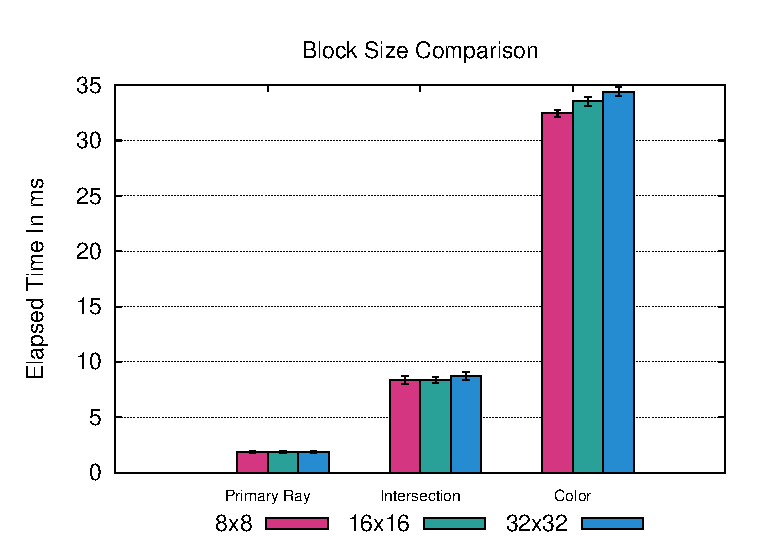
\includegraphics[width=1.0\columnwidth]{Figures/blocksize.eps}
    \caption{Average elapsed time in ms for different block sizes. \label{fig:blockSize}}
\end{figure}

\begin{table}[h!btp]
\centering
\begin{tabular}{c|c|c|c|c}
    Block Size & Primary Ray & Intersection & Color & Total \\ [2pt]
\hline
    8x8 & 1.83612 & 8.37162 & 32.4559 & 42.66364 \\
\hline
    16x16 & 1.86027 & 8.38811 & 33.5634 & 43.81178 \\
\hline
    32x32 & 1.82558 & 8.73071 & 34.4105 & 44.96679 \\
\hline
% Mean Value, Standard Deviation
\end{tabular}
\caption{Average elapsed time in ms for different thread block sizes. \label{tab:ResultsThreadBlockSize}}
\end{table}


\subsection{Triangles}

\begin{figure}[h!tbp]
    \centering
    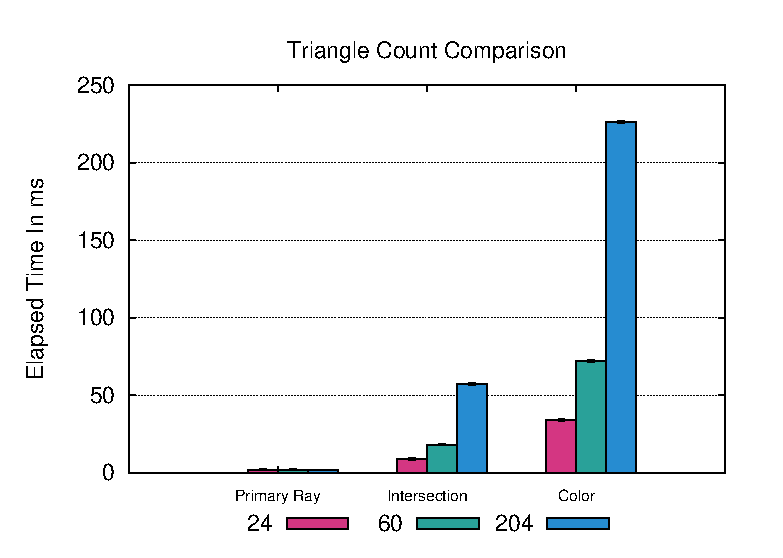
\includegraphics[width=1.0\columnwidth]{Figures/trianglecount.eps}
    \caption{Average elapsed time in ms for different number of triangles. \label{fig:trianglecount}}
\end{figure}

\begin{table}[h!btp]
\centering
\begin{tabular}{c|c|c|c|c}
    Triangle Count & Primary Ray & Intersection & Color & Total \\ [2pt]
\hline
    24  & 1.88325 & 8.87787  & 33.7375 & 44.49862 \\
\hline
    60  & 1.87335 & 18.1137 & 71.9502 & 91.93725 \\
\hline
    204 & 1.86306 & 57.1424 & 226.121 & 285.12646 \\
\hline
% Mean Value, Standard Deviation
\end{tabular}
\caption{Average elapsed time in ms for different number of triangles. \label{tab:ResultsTriangleCount}}
\end{table}



\section{Conclusion}
\label{sec:Conclusion}

Screen resolution has an impact on all stages of the algorithm. More pixels means more rays to calculate which leads to
more work for all three stages.

Trace depth gives a close to a linear performance increase for the Intersection and Color stage. The two stages does the same things in the same way, the
only difference is how many times they are repeated.

Number of lights only affect the Color stage since this stage is the only one concerned with lighting calculations. The
increased execution time is quite noticeable since for each additional light source there is another round of intersection
tests against all primitives in the scene.

Number of triangles has a high impact on both the Intersection and Color stage. Both perform intersection tests against all
triangles in the scene. There is a higher impact on the Color stage since it performs multiple intersection tests against
each triangle, once for each light source.

Thread block size had little to no impact on the Primary Ray and Intersection stage. Only the Color stage exhibited a distinct
change in execution time when the thread block size was change and performs more effectively with smaller block sizes.

Increasing the number of triangles or light sources has a highly detrimental effect on performance since it increases the
number of intersections tests the algorithm has to perform. As it is right now the application can only render simple scenes
and still remain interactive. Partitioning the geometry into a bounding volume hierarchy would likely allow for more complex scenes
to be rendered while still having an acceptable frame rate.

%A bounding volume hierarchy is would be an effective way of increasing performance by limiting the number intersection tests
%performed.
%
%If statements possible impact on performance. GPU performs poorly on branching paths {\color{red}reference needed}. 


\bibliography{Report}
\bibliographystyle{plain}

\end{document}
